
%% \documentclass[]{report}
\documentclass[preprint,10pt]{sigplanconf}
% The following \documentclass options may be useful:

% preprint      Remove this option only once the paper is in final form.
% 10pt          To set in 10-point type instead of 9-point.
% 11pt          To set in 11-point type instead of 9-point.
% authoryear    To obtain author/year citation style instead of numeric.

% \usepackage[a4paper]{geometry}
\usepackage[dvips]{graphicx}            % to include images
%\usepackage{pslatex}	    % to use PostScript fonts

\begin{document}

%%\special{papersize=8.5in,11in}
%%\setlength{\pdfpageheight}{\paperheight}
%%\setlength{\pdfpagewidth}{\paperwidth}

\conferenceinfo{}{} 
\copyrightyear{2014} 
\copyrightdata{978-1-nnnn-nnnn-n/yy/mm} 
\doi{nnnnnnn.nnnnnnn}

\titlebanner{Draft \#0, April 2014}
\preprintfooter{Draft \#0, April 2014}

\title{Machi: an immutable file store}
\subtitle{High level design \& strawman implementation suggestions \\
          with focus on eventual consistency/''EC'' mode of operation}

\authorinfo{Basho Japan KK}{}

\maketitle

\section{Origins}
\label{sec:origins}

This document was first written during the autumn of 2014 for a
Basho-only internal audience.  Since its original drafts, Machi has
been designated by Basho as a full open source software project.  This
document has been rewritten in 2015 to address an external audience.
Furthermore, discussion of the ``chain manager'' service and of strong
consistency have been moved to a separate document, please see
\cite{machi-chain-manager-design}.

\section{Abstract}
\label{sec:abstract}

Our goal
is creation of a robust \& reliable, distributed, highly
available\footnote{Capable of operating in ``AP mode'' or 
  ``CP mode'' relative to the CAP Theorem, see
  Section~\ref{sub:wedge}.}
large file
store based upon write-once registers, append-only files,
Chain Replication, and
client-server style architecture.  All
members of the cluster store all of the files.  Distributed load
balancing/sharding of files is {\em outside} of the scope of this system.
However, it is a high priority that this system be able to integrate
easily into systems that do provide distributed load balancing, e.g.,
Riak Core.  Although strong consistency is a major feature of Chain
Replication, this document will focus mainly on eventual consistency
features --- strong consistency design will be discussed in a separate
document.

\section{Introduction}
\label{sec:introduction}

\begin{quotation}
``I must not scope creep. Scope creep is the mind-killer. Scope creep
  is the little-death that brings total obliteration. I will face my
  scope.''
\par 
\hfill{--- Fred Hebert, {\tt @mononcqc}}
\end{quotation}
\subsection{Name}
\label{sub:name}

This file store will be called ``Machi''.
``Machi'' is a Japanese word for
``village'' or ``small town''.  A village is a rather self-contained
thing, but it is small, not like a city.

One use case for Machi is for file storage, as-is.  However, as Tokyo
City is built with a huge collection of machis, so then this project
is also designed to work well as part of a larger system, such as Riak
Core.  Tokyo wasn't built in a day, after all, and definitely wasn't
built out of a single village.

\subsection{Assumptions}
\label{sub:assumptions}

Machi is a client-server system.  All servers in a Machi cluster store
identical copies/replicas of all files, preferably large files.
\begin{itemize}
    \item This puts an effective limit on the size of a Machi cluster.
      For example, five servers will replicate all files
      for an effective replication $N$ factor of 5.
    \item Any mechanism to distribute files across a subset of Machi
      servers is outside the scope of Machi and of this design.
\end{itemize}

``Large file'' is intended to mean hundreds of MBytes or more
per file.  The design ``sweet spot'' targets about
1 GByte/file and/or managing up to a few million files in a
single cluster.  The maximum size of a single Machi file is
limited by the server's underlying OS and file system; a
practical estimate is 2Tbytes or less but may be larger.

Machi files are write-once, read-many data structures; the label
``append-only'' is mostly correct.  However, to be 100\% truthful
truth, the bytes a Machi file can be written in any order.

Machi files are always named by the server; Machi clients have no
direct control of the name assigned by a Machi server.  Machi servers
specify the file name and byte offset to all client write requests.
(Machi clients may advise servers with a desired file name prefix.)

Machi is not a Hadoop file system (HDFS) replacement.
%% \begin{itemize}
%    \item 
There is no mechanism for writing Machi files to a subset of
      available storage servers: all servers in a Machi server store
      identical copies/replicas of all files.
%    \item 
However, Machi is intended to play very nicely with a layer above it,
      where that layer {\em does} handle file scattering and on-the-fly
      file migration across servers and all of the nice things that
      HDFS, Riak CS, and similar systems can do.

Robust and reliable means that Machi will not lose data until a
fundamental assumption has been violated, e.g., all servers have
crashed permanently.  Machi's file replicaion algorithms can provide
strong or eventual consistency and is provably correct.  Our only
task is to not put bugs into the implementation of the algorithms.  Machi's
small pieces and restricted API and semantics will reduce
(we believe) the effort required to test
and verify the implementation.

Machi should not have ``big'' external runtime dependencies when
practical.  For example, the feature set of ZooKeeper makes it a
popular distributed systems coordination service.  When possible,
Machi should try to avoid using such a big runtime dependency.  For
the purposes of explaining ``big'', the Riak KV service is too big and
thus runs afoul of this requirement.

Machi clients must assume that any interrupted or incomplete write
operation may be readable at some later time.  Read repair or
incomplete writes may happen long after the client has finished or
even crashed.  In effect, Machi will provide clients with
``at least once'' behavior for writes.

\subsection{Defining a Machi file}

A Machi ``file'' is an undifferentiated, one-dimensional array of
bytes.  This definition matches the POSIX definition of a file.
However, the Machi API does not conform to the UNIX/POSIX file
I/O API.

A list of client operations are shown in
Figure~\ref{fig:example-client-API}.  This list may change, but it
shows the basic shape of the service.

\begin{figure}
\begin{itemize}
        \item Append bytes $B$ to a file with name prefix {\tt "foo"}.
        \item Read $N$ bytes from offset $O$ from file $F$.
        \item List files: name, size, etc.
\end{itemize}
\caption{Full (?) list of file API operations}
\label{fig:example-client-API}
\end{figure}

The file read \& write granularity of Machi is one byte.  (In CORFU
operation mode, perhaps, the granularity would be page size on the
order of 4 KBytes or 16 KBytes.)

\begin{figure}
    \begin{enumerate}
        \item Client1: Write 1 byte at offset 0.
        \item Client1: Read 1 byte at offset 0.
        \item Client2: Write 1 byte at offset 2.
        \item Client2: Read 1 byte at offset 2.
        \item Client3: (an intermittently slow client) Write 1 byte at offset 1.
        \item Client3: Read 1 byte at offset 1.
    \end{enumerate}
\caption{Example of temporally out-of-order file append sequence that
  is valid within a Machi cluster.}
\label{fig:temporal-out-of-order}
\end{figure}

\subsubsection{Append-only files}
\label{sub:assume-append-only}

Machi's file writing semantics are append-only.  
Machi's append-only behavior is spatial and is {\em not}
enforced temporally.  For example, Figure~\ref{fig:temporal-out-of-order}
shows client operations
upon a single file, in strictly increasing wall clock time ticks.
Figure~\ref{fig:temporal-out-of-order}'s is perfectly valid Machi behavior.

%% In this example, client 3 was
%% very quick and was actually the second client to request
%% appending to the file and therefore was assigned to write to
%% offset \#1.  However, client 3 then became slow and didn't
%% actually write its data to offset 1 until after step 4.

Any byte in a file may have three states:
\begin{enumerate}
    \item unwritten: no value has been assigned to the byte.
    \item written: exactly one value has been assigned to the byte.
    \item trimmed: only used for garbage collection \& disk space
      reclamation purposes
\end{enumerate}

Transitions between these states are strictly ordered.  Valid
orders are:
    \begin{itemize}
        \item unwritten $\rightarrow$ written
        \item unwritten $\rightarrow$ trimmed
        \item written $\rightarrow$ trimmed
    \end{itemize}
%% The trim operation may be used internally to mark byte ranges
%% which have been marked ``no longer in use'', e.g. with a reference
%% count of zero.  Such regions may be garbage collected by Machi
%% at its convenience.\footnote{Advanced feature, implementation TBD.}

Client append operations are atomic: the transition from
one state to another happens for all bytes, or else no
transition is made for any bytes.

\subsubsection{Machi servers choose all file names}

A Machi server always chooses the full file name of file
  that will have data appended to it.
A Machi server always chooses the offset within the file
  that will have data appended to it.

All file names chosen by Machi are unique, relative to itself.  Any
duplicate file names can cause correctness violations.\footnote{For
  participation in a larger system, Machi can construct file names that
  are unique within that larger system, e.g. by embedding a unique
  Machi cluster name or perhaps a UUID-style
  string in the name.}

\subsubsection{File integrity and bit-rot}
\label{sub:bit-rot}

Clients may specify a per-write checksum of the data being written,
e.g., SHA1.  These checksums will be appended to the file's
metadata.  Checksums are first-class metadata and is replicated with
the same consistency and availability guarantees as its corresponding
file data.
Clients may optionally fetch the checksum of the bytes they
read.

Bit-rot can and will happen.  To guard against bit-rot on disk, strong
  checksums are used to detect bit-rot at all possible places.
\begin{itemize}
    \item Client-calculated checksums of appended data
    \item Whole-file checksums, calculated by Machi servers for internal
      sanity checking.  See \ref{sub:detecting-corrupted} for
      commentary on how this may not be feasible.
    \item Any other place that makes sense for the paranoid.
\end{itemize}

Full 100\% protection against arbitrary RAM bit-flips is not a design
goal \ldots but would be cool for as research for the great and
glorious future.  Meanwhile, Machi will use as many ``defense in
depth'' techniques as feasible.

\subsubsection{File metadata}

Files may have metadata associated with them.
Clients may request appending metadata to a file, for example,
  {\tt \{file F, bytes X-Y, property list of 2-tuples\}}.
This metadata receives second-class handling with regard to
consistency and availability, as described below and in contrast to
the per-append checksums described in Section~\ref{sub:bit-rot}

\begin{itemize}
    \item File metadata is strictly append-only.
    \item File metadata is always eventually consistent.
    \item A complete history of all metadata updates is maintained for
      each file.  
    \item Temporal order of metadata entries is not preserved.
    \item Multiple histories for a file may be merged at any time.
    \begin{itemize}
        \item If a client requires idempotency, then the property list
          should contain all information required to identify multiple
          copies of the same metadata item.
        \item Metadata properties should be considered CRDT-like: the
          final metadata list should converge eventually to a single
          list of properties. 
    \end{itemize}
\end{itemize}

\subsubsection{File replica management via Chain Replication}
\label{sub:chain-replication}

Machi uses Chain Replication (CR) internally to maintain file
replicas and inter-replica consistency.
A Machi cluster of $F+1$ servers can sustain the failure of up
to $F$ servers without data loss.

A simple explanation of Chain Replication is that it is a variation of
single-primary/multiple-secondary replication with the following
restrictions:

\begin{enumerate}
\item All writes are strictly performed by servers that are arranged
  in a single order, known as the ``chain order'', beginning at the
  chain's head.
\item All strongly consistent reads are performed only by the tail of
  the chain, i.e., the last server in the chain order.
\item Inconsistent reads may be performed by any single server in the
  chain.
\end{enumerate}

Machi contains enough Chain Replication implementation to maintain its
chain state, file data integrity, and file metadata eventual
consistency.  See also Section~\ref{sub:self-management}.

The first version of Machi would use a single chain for managing all
files in the cluster.  If the system is quiescent,
then all chain members store the same data: all
Machi servers will all store identical files.  Later versions of Machi
may play clever games with projection data structures and algorithms
that interpret these projections to implement alternative replication
schemes.  However, such clever games are scope creep and are therefore
research topics for the future.

Machi will probably not\footnote{Final decision TBD} implement chain
replication using CORFU's description of its protocol.  CORFU's
authors made an implementation choice to make the FLU servers
(Section~\ref{sub:flu}) as dumb as possible.  The CORFU authors were
(in part) experimenting with the FLU server implemented by an FPGA; a
dumb-as-possible server was a feature.

Machi does not have CORFU's minimalism as a design principle.
Therefore, it's likely that Machi will implement CR using the original
Chain Replication \cite{chain-replication} paper's pattern of message
passing, i.e., with direct server-to-server message
passing.\footnote{Also, the original CR algorithm's requirement for
  message passing back up the chain to enforce write consistency is
  not required: Machi's combination of client-driven data repair and
  write-once registers make inter-server synchronization unnecessary.}
However, the
description of the protocols in this document will use CORFU-style
Chain Replication.  The two variations are equivalent from a
correctness point of view --- what matters is the communication
pattern and total number of messages required per operation.
CORFU's
client-driven messaging patterns feel easier to describe and to
align with CORFU- and Tango-related research papers.

\subsubsection{Data integrity self-management}
\label{sub:self-management}

Machi servers automatically monitor each others health.  Signs
of poor health will automatically reconfigure the Machi cluster
to avoid data loss and to provide maximum availability.
For example, if a server $S$ crashes and later
restarts, Machi will automatically bring the data on $S$ back to full sync.

Machi will provide an administration API for managing Machi servers, e.g.,
cluster membership, file integrity and checksum verification, etc.

%% Machi's use of Chain Replication internally means that certain
%% combinations of server $S$ fails, $S$ restarts, recovery repair $R_s$
%% starts to repair $S$'s data, 
%% and a separate failure happen before the $R_s$ repair has
%% completed ... can lead to data loss.  Such data loss events will
%% be avoided by fail-stop behavior of the entire Machi cluster
%% until external/human intervention can restart nodes that contain
%% at-risk-of-loss data.

%% All of Machi's participants, client and server alike, fully observe
%% Machi's protocols, write-once enforcement, projection changes (see
%% below), ``wedge'' enforcement (see below), etc.

\subsection{Out of Machi's scope}

Anything not mentioned in this paper is outside of Machi's scope.
However, it's worth mentioning (again!) that the following are explicitly
considered out-of-scope for Machi.

  Machi does not distribute/shard files across disjoint sets of servers.
  Distribution of files across Machi servers is left for a higher
  level of abstraction, e.g. Riak Core.  See also
  Sections~\ref{sub:name} and \ref{sub:assumptions} and the quote at
  the top of Section~\ref{sec:introduction}.

  Later versions of Machi may support erasure
  coding directly, or Machi can be used as-is to store files that
  client applications that are aware that they are manipulating
  erasure coded data.  In the latter case,
  the client can read a 1 GByte file from a Machi cluster with a chain
  length of $N$, erasure encode it in a
  15-choose-any-10 encoding scheme and concatenate them into a 1.5 GByte file,
  then store each of the fifteen
  0.1 GByte chunks in a different Machi cluster, each with a chain
  length of only $1$.  Using separate Machi clusters makes the
  burden of physical separation of each coded piece (i.e., ``rack
  awareness'') someone/something else's problem.

Why would would someone wish to run a Machi cluster with only one
server (i.e., chain length of one) rather than using the FLU service
(Section~\ref{sub:flu}) by itself?  One answer is that data
migration is much easier with all of Machi than with only the FLU
server.  To migrate all files from FLU $F_a$ to FLU $F_b$, the administrator
merely needs to add $F_b$ to the end of $F_a$'s chain.  When the data
repair is finished, we know that $F_b$ stores full replicas of all of
$F_a$'s data.  The administrator removes $F_a$ from the chain, and the
data migration is finished.

\section{Architecture: base components and ideas}

This section presents the major architectural components.  They are:

\begin{itemize}
\item The FLU: the server that stores a single replica of a file.
(Section \ref{sub:flu})
\item The Sequencer: assigns a unique file name + offset to each file
  append request.
(Section \ref{sub:sequencer})
\item The Projection Store: a write-once key-value blob store, used by
  Machi for storing projections.
(Section \ref{sub:proj-store})
\item The chain manager: monitors the health of the
  chain and calculates new projections when failure is detected.
(Section \ref{sub:chain-manager})
\end{itemize}

Also presented here are the major concepts used by Machi components:
\begin{itemize}
\item The Projection: the data structure that describes the current
  state of the Machi chain.  
  and is stored in the write-once Projection Store.
(Section \ref{sub:projection})
\item The Projection Epoch Number (a.k.a.~The Epoch): Each projection
  is numbered with an epoch.
(Also section \ref{sub:projection})
\item The Bad Epoch Error: a response when a protocol operation uses a
  projection epoch number smaller than the current projection epoch.
(Section \ref{sub:bad-epoch})
\item The Wedge: a response when a protocol operation uses a
  projection epoch number larger than the current projection epoch.
(Section \ref{sub:wedge})
\item AP Mode and CP Mode: the general mode of a Machi cluster may be
  in ``AP Mode'' or ``CP Mode'', which are short-hand notations for
  Machi clusters with eventual consistency or strong consistency
  behavior.  Both modes have different availability profiles and
  slightly different feature sets.  (Section \ref{sub:ap-cp-mode})
\end{itemize}

\subsection{The FLU}
\label{sub:flu}

The basic idea of the FLU is borrowed from CORFU.  The base CORFU
data server is called a ``flash unit''.  For Machi, the equivalent
server is nicknamed a FLU, a ``FiLe replica Unit''.  A FLU is
responsible for maintaining a single replica/copy of each file
(and its associated metadata) stored in a Machi cluster

The FLU's API is very simple: see Figure~\ref{fig:flu-api} for its
data types and operations.  This description is not 100\% complete but
is sufficient for discussion purposes.

\begin{figure*}[]
\begin{verbatim}
-type m_bytes()     :: iolist().
-type m_csum()      :: {none | sha1 | sha1_excl_final_20, binary(20)}.
-type m_epoch()     :: {m_epoch_n(), m_csum()}.
-type m_epoch_n()   :: non_neg_integer().
-type m_err_r()     :: error_unwritten | error_trimmed.
-type m_err_w()     :: error_written | error_trimmed.
-type m_file_info() :: {m_name(), Size::integer(), ...}.
-type m_fill_err()  :: error_not_permitted.
-type m_generr()    :: error_bad_epoch | error_wedged |
                       error_bad_checksum | error_unavailable.
-type m_name()      :: binary().
-type m_offset()    :: non_neg_integer().
-type m_rerror()    :: m_err_r() m_generr().
-type m_werror()    :: m_generr() | m_err_w().

-spec fill(m_name(),  m_offset(), integer(), m_epoch()) -> ok | m_fill_err() |
                                                           m_werror().
-spec list_files()                                      -> {ok, [m_file_info()]} | m_generr().
-spec read(m_name(),  m_offset(), integer(), m_epoch()) -> {ok, binary()} | m_rerror().
-spec trim(m_name(),  m_offset(), integer(), m_epoch()) -> ok | m_generr().
-spec write(m_name(), m_offset(), m_bytes(), m_csum(),
                                             m_epoch()) -> ok | m_werror().

-spec proj_get_largest_key()                            -> m_epoch_n() | error_unavailable.
-spec proj_get_largest_keyval()                         -> {ok, m_epoch_n(), binary()} |
-spec proj_list()                                       -> {ok, [m_epoch_n()]}.
-spec proj_read(m_epoch_n())                            -> {ok, binary()} | m_err_r().
-spec proj_write(m_epoch_n(), m_bytes(), m_csum())      -> ok | m_err_w() |
                                                           error_unwritten | error_unavailable. 
\end{verbatim}
\caption{FLU data and projection operations as viewed as an API and data types (excluding metadata operations)}
\label{fig:flu-api}
\end{figure*}

The FLU must enforce the state of each byte of each file.
Transitions between these states are strictly ordered.
See Section~\ref{sub:assume-append-only} for state transitions and
the restrictions related to those transitions.

The FLU also keeps track of the projection number (number and checksum
both, see also Section~\ref{sub:flu-divergence}) of the last modification to a
file.  This projection number is used for quick comparisons during
repair (Section~\ref{sec:repair}) to determine if files are in sync or
not.

\subsubsection{Divergence from CORFU}
\label{sub:flu-divergence}

In Machi, the type signature of {\tt
  m\_epoch()} includes both the projection epoch number and a checksum
of the projection's contents.  This checksum is used in cases where
Machi is configured to run in ``AP mode'', which allows a running Machi
cluster to fragment into multiple running sub-clusters during network
partitions.  Each sub-cluster can choose a projection number
$P_{side}$ for its side of the cluster.

After the partition is
healed, it may be true that epoch numbers assigned to two different
projections $P_{left}$ and  $P_{right}$
are equal.  However, their checksum signatures will differ.  If a
Machi client or server detects a difference in either the epoch number
or the epoch checksum, it must wedge itself (Section~\ref{sub:wedge})
until a new projection with a larger epoch number is available.

\subsection{The Sequencer}
\label{sub:sequencer}

For every file append request, the Sequencer assigns a unique
{\tt \{file-name,byte-offset\}} location tuple.

Each FLU server runs a sequencer server.  Typically, only the
sequencer of the head of the chain is used by clients.  However, for
development and administration ease, each FLU should have a sequencer
running at all times.  If a client were to use a sequencer other than
the chain head's sequencer, no harm would be done.

The sequencer must assign a new file name whenever any of the
following events happen:
\begin{itemize}
\item The current file size is too big, per cluster administration policy.
\item The sequencer or the entire FLU restarts.
\item The FLU receives a projection or client API call
  that includes a newer/larger projection epoch
  number than its current projection epoch number.
\end{itemize}

The sequencer assignment given to a Machi client is valid only for the
projection epoch in which it was assigned.  Machi FLUs must enforce
this requirement.  If a Machi client's write attempt is interrupted in
the middle by a projection change, then the following rules must be
used to continue:

\begin{itemize}
\item If the client's write has been successful on at least the head
  FLU in the chain, then the client may continue to use the old
  location.  The client is now performing read repair of this location in
  the new epoch.  (The client may have to add a ``read repair'' option
  to its requests to bypass the FLUs usual enforcement of the
  location's epoch.)
\item If the client's write to the head FLU has not started yet, or if
  it doesn't know the status of the write to the head (e.g., timeout),
  then the client must abandon the current location assignment and
  request a new assignment from the sequencer.
\end{itemize}

\subsubsection{Divergence from CORFU}
\label{sub:sequencer-divergence}

CORFU's sequencer is not
necessary in a CORFU system and is merely a performance optimization.  

In Machi, the sequencer is required because it assigns both a file
byte offset and also a full file name.  The client can request a
certain file name prefix, e.g. {\tt "foo"}.  The sequencer must make
the file name unique across the entire Machi system.  A Machi cluster
has a name that is shared by all servers.  The client's prefix
wish is combined with the cluster name, sequencer name, and a
per-sequencer strictly unique ID (such as a counter) to form an opaque
suffix.
For example,
\begin{quote}
{\tt "foo.m=machi4.s=flu-A.n=72006"}
\end{quote}

One reviewer asked, ``Why not just use UUIDs?''  Any naming system
that generates unique file names is sufficient.

\subsection{The Projection Store}
\label{sub:proj-store}

Each FLU maintains a key-value store for the purpose of storing
projections.  Reads \& writes to this store are provided by the FLU
administration API.  The projection store runs on each server that
provides FLU service, for two reasons of convenience.  First, the
projection data structure
need not include extra server names to identify projection
store servers or their locations.
Second, writes to the projection store require
notification to a FLU of the projection update anyway.

The store's basic operation set is simple: get, put, get largest key
(and optionally its value), and list all keys.
The projection store's data types are:

\begin{itemize}
\item key = the projection number
\item value = the entire projection data structure, serialized as an
  opaque byte blob stored in write-once register. The value is 
  typically a few KBytes but may be up to 10s of MBytes in size.
  (A Machi projection data structure will likely be much less than 10
  KBytes.)
\end{itemize}

As a write-once register, any attempt to write a key $K$ when the
local store already has a value written for $K$ will always fail
with a {\tt error\_written} error.

Any write of a key whose value is larger than the FLU's current
projection number will move the FLU to the wedged state
(Section~\ref{sub:wedge}).

The contents of the projection blob store are maintained by neither
Chain Replication techniques nor any other server-side technique.  All
replication and read repair is done only by the projection store
client.  Astute readers may theorize that race conditions exist in
such management; see Section~\ref{sec:projections} for details and
restrictions that make it practical.

\subsection{The chain manager}
\label{sub:chain-manager}

Each FLU runs an administration agent that is responsible for
monitoring the health of the entire Machi cluster.  If a change of
state is noticed (via measurement) or is requested (via the
administration API), zero or more actions may be taken:

\begin{itemize}
\item Enter wedge state (Section~\ref{sub:wedge}).
\item Calculate a new projection to fit the new environment.
\item Attempt to store the new projection locally and remotely.
\item Read a newer projection from local + remote stores (and possibly
  perform read repair).
\item Adopt a new unanimous projection, as read from all
  currently available readable blob stores.
\item Exit wedge state.
\end{itemize}

See also Section~\ref{sec:projections} and also the Chain Manager
design document \cite{machi-chain-manager-design}.

\subsection{The Projection and the Projection Epoch Number}
\label{sub:projection}

The projection data
structure defines the current administration \& operational/runtime
configuration of a Machi cluster's single Chain Replication chain.
Each projection is identified by a strictly increasing counter called
the Epoch Projection Number (or more simply ``the epoch'').

\begin{figure}
\begin{verbatim}
-type m_server_info() :: {Hostname, Port,...}.
-record(projection, {
            epoch_number    :: m_epoch_n(),
            epoch_csum      :: m_csum(),
            creation_time   :: now(),
            author_server   :: m_server(),
            all_members     :: [m_server()],
            active_upi      :: [m_server()],
            active_all      :: [m_server()],
            down_members    :: [m_server()],
            dbg_annotations :: proplist()
        }).
\end{verbatim}
\caption{Sketch of the projection data structure}
\label{fig:projection}
\end{figure}

Projections are calculated by each FLU using input from local
measurement data, calculations by the FLU's chain manager
(see below), and input from the administration API.
Each time that the configuration changes (automatically or by
administrator's request), a new epoch number is assigned
to the entire configuration data structure and is distributed to
all FLUs via the FLU's administration API.  Each FLU maintains the
current projection epoch number as part of its soft state.

Pseudo-code for the projection's definition is shown in
Figure~\ref{fig:projection}.  To summarize the major components:

\begin{itemize}
\item {\tt creation\_time} Wall-clock time, useful for humans and
  general debugging effort.
\item {\tt author\_server} Name of the server that calculated the projection.
\item {\tt all\_members} All servers in the chain, regardless of current
  operation status.  If all operating conditions are perfect, the
  chain should operate in the order specified here.
  (See also the limitations in \cite{machi-chain-manager-design},
  ``Whole-file repair when changing FLU ordering within a chain''.)
\item {\tt active\_upi} All active chain members that we know are
  fully repaired/in-sync with each other and therefore the Update
  Propagation Invariant \cite{machi-chain-manager-design} is always true.
  See also Section~\ref{sec:repair}.
\item {\tt active\_all} All active chain members, including those that
  are under active repair procedures.
\item {\tt down\_members} All members that the {\tt author\_server}
  believes are currently down or partitioned.
\item {\tt dbg\_annotations} A ``kitchen sink'' proplist, for code to
  add any hints for why the projection change was made, delay/retry
  information, etc.
\end{itemize}

\subsection{The Bad Epoch Error}
\label{sub:bad-epoch}

Most Machi protocol actions are tagged with the actor's best knowledge
of the current epoch.  However, Machi does not have a single/master
coordinator for making configuration changes.  Instead, change is
performed in a fully asynchronous manner.  During a cluster
configuration change, some servers will use the old projection number,
$P_p$, whereas others know of a newer projection, $P_{p+x}$ where $x>0$.

When a protocol operation with $P_p$ arrives at an actor who knows
$P_{p+x}$, the response must be {\tt error\_bad\_epoch}.  This is a signal
that the actor using $P_p$ is indeed out-of-date and that a newer
projection must be found and used.

\subsection{The Wedge}
\label{sub:wedge}

If a FLU server is using a projection $P_p$ and receives a protocol
message that mentions a newer projection $P_{p+x}$ that is larger than its
current projection value, then it must enter ``wedge'' state and stop
processing all new requests.  The server remains in wedge state until
a new projection (with a larger/higher epoch number) is discovered and
appropriately acted upon.
In the Windows Azure storage system \cite{was}, this state is called
the ``sealed'' state.

\subsection{``AP Mode'' and ``CP Mode''}
\label{sub:ap-cp-mode}

Machi's first use cases require only eventual consistency semantics
and behavior, a.k.a.~``AP mode''.  However, with only small
modifications, Machi can operate in a strongly consistent manner,
a.k.a.~``CP mode''.

The chain manager service (Section \ref{sub:chain-manager}) is
sufficient for an ``AP Mode'' Machi service.  In AP Mode, all mutations
to any file on any side of a network partition are guaranteed to use
unique locations (file names and/or byte offsets).  When network
partitions are healed, all files can be merged together
(while considering the file format detail discussed in
the footnote of Section~\ref{ssec:just-rsync-it}) in any order
without conflict.

``CP mode'' will be extensively covered in other documents.  In summary,
to support ``CP mode'', we believe that the chain manager
service proposed here can guarantee strong consistency
at all times.

\section{Sketches of single operations}
\label{sec:sketches}

\subsection{Single operation: append a single sequence of bytes to a file}
\label{sec:sketch-append}

%% NOTE: append-whiteboard.eps was created by 'jpeg2ps'.
\begin{figure*}[htp]
\resizebox{\textwidth}{!}{
	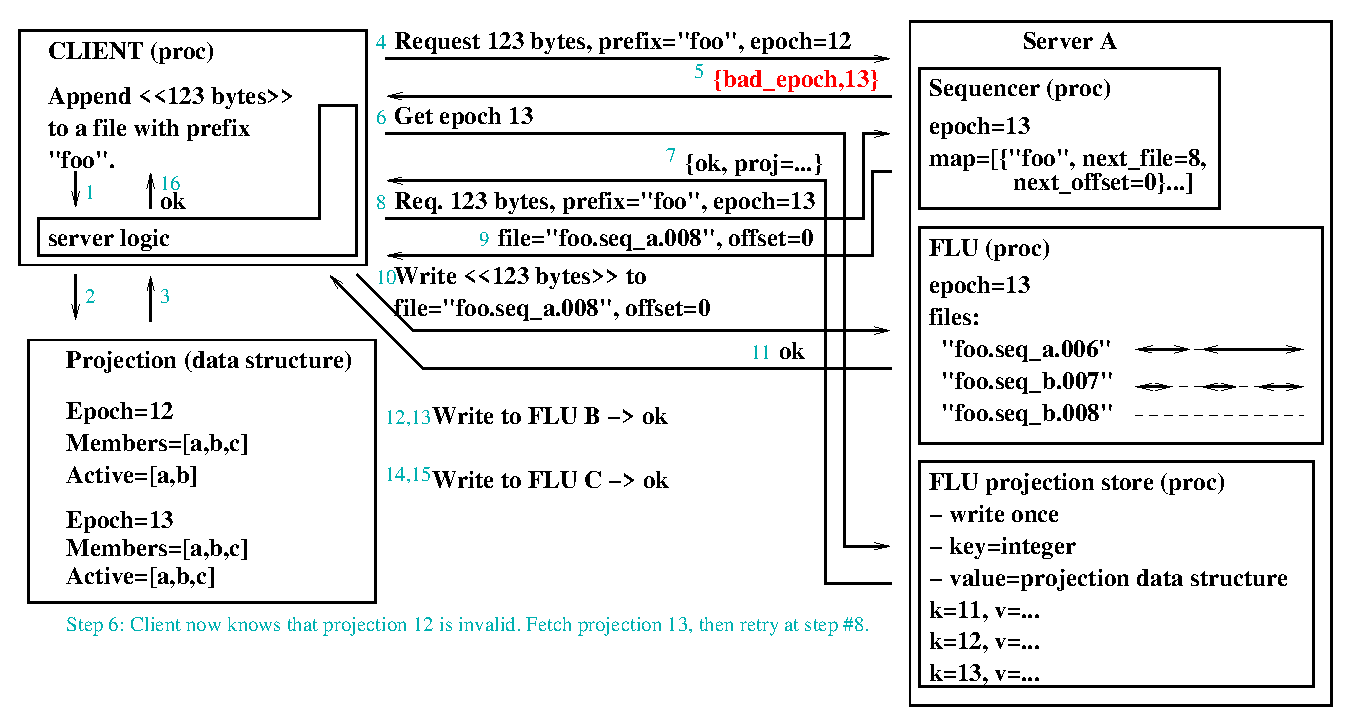
\includegraphics[width=\textwidth]{figure6}
	%% \includegraphics[width=\textwidth]{append-whiteboard}
	}
\caption{Flow diagram: append 123 bytes onto a file with prefix {\tt "foo"}.}
\label{fig:append-flow}
\end{figure*}

To write/append atomically a single sequence/hunk of bytes to a file,
here's the sequence of steps required.
See Figure~\ref{fig:append-flow} for a diagram showing an example
append; the same example is also shown in
Figure~\ref{fig:append-flowMSC} using MSC style (message sequence chart).
In
this case, the first FLU contacted has a newer projection epoch,
$P_{13}$, than the $P_{12}$ epoch that the client first attempts to use.

\begin{enumerate}

\item The client chooses a file name prefix.  This prefix gives the
sequencer implicit advice of where the client wants data to be
placed.  For example, if two different append requests are for file
prefixes $Pref1$ and $Pref2$ where $Pref1 \ne Pref2$, then the two byte
sequences will definitely be written to different files.  If
$Pref1 = Pref2$,
then the sequencer may choose the same file for both (but no
guarantee of how ``close together'' the two requests might be).

\item (cacheable) Find the list of Machi member servers.  This step is
only needed at client initialization time or when all Machi members
are down/unavailable.  This step is out of scope of Machi, i.e., found
via another source: local configuration file, DNS, LDAP, Riak KV, ZooKeeper,
carrier pigeon, etc.

\item (cacheable) Find the current projection number and projection data
structure by fetching it from one of the Machi FLU server's
projection store service.  This info
may be cached and reused for as long as Machi server requests do not
result in {\tt error\_bad\_epoch}.

\item Client sends a sequencer op to the sequencer process on the head of
the Machi chain (as defined by the projection data structure):
{\tt \{sequence\_req, Filename\_Prefix, Number\_of\_Bytes\}}.  The reply
includes {\tt \{Full\_Filename, Offset\}}.

\item The client sends a write request to the head of the Machi chain:
{\tt \{write\_req, Full\_Filename, Offset, Bytes, Options\}}.  The
client-calculated checksum is a recommended option.

\item If the head's reply is {\tt ok}, then repeat for all remaining chain
members in strict chain order.

\item If all chain members' replies are {\tt ok}, then the append was
successful.  The client now knows the full Machi file name and byte
offset, so that future attempts to read the data can do so by file
name and offset.

\item Upon any non-{\tt ok} reply from a FLU server, {\em the client must
consider the entire append operation a failure}.  If the client
wishes, it may retry the append operation using a new location
assignment from the sequencer or, if permitted by Machi restrictions,
perform read repair on the original location.  If this read repair is
fully successful, then the client may consider the append operation
successful.

\item If a FLU server $FLU$ is unavailable, notify another up/available
chain member that $FLU$ appears unavailable.  This info may be used by
the chain manager service to change projections.  If the client
wishes, it may retry the append op or perhaps wait until a new projection is
available.

\item If any FLU server reports {\tt error\_written}, then either of two
things has happened:
\begin{itemize}
    \item The appending client $C_w$ was too slow when attempting to write
    to the head of the chain.
    Another client, $C_r$, attempted a read, noticed that the tail's value was
    unwritten and noticed that the head's value was also unwritten.
    Then $C_r$ initiated a ``fill'' operation to write junk into
    this offset of
    the file.  The fill operation succeeded, and now the slow
    appending client $C_w$ discovers that it was too slow via the
    {\tt error\_written} response.
    \item The appending client $C_w$ was too slow after at least one
    successful write. 
    Client $C_r$ attempted a read, noticed the partial write, and
    then engaged in read repair.  Client $C_w$ should also check all
    replicas to verify that the repaired data matches its write
    attempt -- in all cases, the values written by $C_w$ and $C_r$ are
    identical.
\end{itemize}

\end{enumerate}

\subsection{TODO: Single operation: reading a chunk of bytes from a file}
\label{sec:sketch-read}

\section{Projections: calculation, then storage, then (perhaps) use}
\label{sec:projections}

Machi uses a ``projection'' to determine how its Chain Replication replicas
should operate; see Section~\ref{sub:chain-replication} and
\cite{corfu1}.  At runtime, a cluster must be able to respond both to
administrative changes (e.g., substituting a failed server box with
replacement hardware) as well as local network conditions (e.g., is
there a network partition?).  The concept of a projection is borrowed
from CORFU but has a longer history, e.g., the Hibari key-value store
\cite{cr-theory-and-practice} and goes back in research for decades,
e.g., Porcupine \cite{porcupine}.

See \cite{machi-chain-manager-design} for the design and discussion of
all aspects of projection management and storage.

\section{Chain Replication repair: how to fix servers after they crash
and return to service}
\label{sec:repair}

%% Section~\ref{sec:safety-of-transitions} mentions that there are some
%% not-obvious ways that a Machi cluster could inadvertently lose data.
%% It is possible to avoid data loss in all cases, short of all servers
%% being destroyed by a fire.
The theory of why it's possible to avoid
data loss with chain replication is summarized in this section,
followed by a discussion of Machi-specific details that must be
included in any production-quality implementation.

\subsection{When to trigger read repair of single values}

Assume now that some client $X$ wishes to fetch a datum that's managed
by Chain Replication.  Client $X$ must discover the chain's
configuration for that datum, then send its read request to the tail
replica of the chain, $R_{tail}$.

In CORFU and in Machi, the store is a set of write-once registers.
Therefore, the only possible responses that client $X$ might get from a
query to the chain's $R_{tail}$ are:

\begin{enumerate}
\item {\tt error\_unwritten}
\item {\tt \{ok, <<...data bytes...>>\}}
\item {\tt error\_trimmed} (in environments where space
  reclamation/garbage collection is permitted)
\end{enumerate}

Let's explore each of these responses in the following subsections.

\subsubsection{Tail replica replies {\tt error\_unwritten}}

There are only a few reasons why this value is possible.  All are
discussed here.

\paragraph{Scenario 1: The block truly hasn't been written yet}

A read from any other server in the chain will also yield {\tt
  error\_unwritten}.

\paragraph{Scenario 2: The block has not yet finished being written}

A read from any other server in the chain may yield {\tt
  error\_unwritten} or may find written data.  (In this scenario, the
head server has written data; we don't know the state of the middle
and tail server(s).)  The client ought to perform read repair of this
data.  (See also, scenario \#4 below.)

During read repair, the client's writes operations may race with the
original writer's operations.  However, both the original writer and
the repairing client are always writing the same data.  Therefore,
data corruption by conflicting client writes is not possible.  

\paragraph{Scenario 3: A client $X_w$ has received a sequencer's
  assignment for this
  location, but the client has crashed somewhere in the middle of
  writing the value to the chain.}

The correct action to take here depends on the value of the $R_{head}$
replica's value.  If $R_{head}$'s value is unwritten, then the writing
client $X_w$ crashed before writing to $R_{head}$.  The reading client
$X_r$ must ``fill'' the page with junk bytes or else do nothing.

If $R_{head}$'s value is indeed written, then the reading client $X_r$
must finish a ``read repair'' operation before the client may proceed.
See Section~\ref{sub:read-repair-single} for details.

\paragraph{Scenario 4: A client has received a sequencer's assignment for this
  location, but the client has become extremely slow (or is
  experiencing a network partition, or any other reason) and has not
  yet updated $R_{tail}$ $\ldots$ but that client {\em will eventually
    finish its work} and will eventually update $R_{tail}$.}

It should come as little surprise that reading client $C_r$
cannot know whether the writing client $C_w$
has really crashed or if $C_w$ is merely very slow.
It is therefore very nice that
the action that $C_r$ must take in either case is the same --- see the
scenario \#2 for details.

\subsubsection{Tail replica replies {\tt \{ok, <<...>>\}}}

There is no need to perform single item read repair in this case.
The Update Propagation Invariant guarantees that this value is the one
strictly consistent value for this register.

\subsubsection{Tail replica replies {\tt error\_trimmed}}

There is no need to perform single item read repair in this case.

{\bf NOTE:} It isn't yet clear how much support early versions of
Machi will need for GC/space reclamation via trimming.

\subsection{How to read repair a single value}
\label{sub:read-repair-single}

If a value at $R_{tail}$ is unwritten, then the answer to ``what value
should I use to repair the chain's value?'' is simple: the value at the
head $R_{head}$ is the value $V_{head}$ that must be used.  The client
then writes $V_{head}$ to all other members of the chain $C$, in
order.

The client may not proceed with its upper-level logic until the read
repair operation is successful.  If the read repair operation is not
successful, then the client must react in the same manner as if the
original read attempt of $R_{tail}$'s value had failed.

\subsection{Repair of entire files}
\label{sub:repair-entire-files}

There are some situations where repair of entire files is necessary.

\begin{itemize}
\item To repair FLUs added to a chain in a projection change,
  specifically adding a new FLU to the chain.  This case covers both
  adding a new, data-less FLU and re-adding a previous, data-full FLU
  back to the chain.
\item To avoid data loss when changing the order of the chain's servers.
\end{itemize}

The full file repair discussion in \cite{machi-chain-manager-design}
argues for correctness in both eventually consistent and strongly
consistent environments.  Discussion in this section will be limited
to eventually consistent environments (``AP mode'') .

\subsubsection{``Just `rsync' it!''}
\label{ssec:just-rsync-it}

The ``just {\tt rsync} it!'' method could loosely be described as,
``run {\tt rsync} on all files to all servers.''  This simple repair
method is nearly sufficient enough for Machi's eventual consistency
mode of operation.  There's only one small problem that {\tt rsync}
cannot handle by itself: handling late writes to a file.  It is
possible that the same file could contain the following pattern of
written and unwritten data:

\begin{itemize}
\item Server $A$: $x$ bytes written, $y$ bytes unwritten
\item Server $B$: $x$ bytes unwritten, $y$ bytes written
\end{itemize}

If {\tt rsync} is uses as-is to replicate this file, then one of the
two written sections will overwritten by NUL bytes.  Obviously, we
don't want this kind of data loss.  However, we already have a
requirement that Machi file servers must enforce write-once behavior
on all file byte ranges.  The same data used to maintain written and
unwritten state can be used to merge file state so that both the $x$
and $y$ byte ranges will be correct after repair.

\subsubsection{The larger problem with ``Just `rsync' it!''}

Assume for a moment that the {\tt rsync} utility could indeed preserve
Machi written chunk boundaries as described above.  A larger
administration problem still remains: this informal method cannot tell
you exactly when you are in danger of data loss or when data loss has
actually happened.  If we maintain the Update Propagation Invariant
(as argued in \cite{machi-chain-manager-design},
then we always know exactly when data loss is immanent or has happened.

\section{On-disk storage and file corruption detection}
\label{sec:on-disk}

An individual FLU has a couple of goals: store file data and metadata
as efficiently as possible, and make it easy to detect and fix file
corruption.

FLUs have a lot of flexibility to implement their on-disk data formats in
whatever manner allow them to be safe and fast.  Any format that
allows safe management of file names, per-file data chunks, and
per-data-chunk metadata is sufficient.

\subsection{First draft/strawman proposal for on-disk data format}
\label{sub:on-disk-data-format}

{\bf NOTE:} The suggestions in this section are ``strawman quality''
only.

\begin{figure*}
\begin{verbatim}
|<--- Data section --->|<---- Metadata section (starts at fixed offset) ---->
                                                          |<- trailer -->
V1,C1 | V2,C2 |       ||| C1t,O1a,O1z,C1 | C2t,O2a,O2z,C2 | Summ | SummBytes |eof
                                                                           |<- trailer -->
V1,C1 | V2,C2 | V3,C3 ||| C1t,O1a,O1z,C1 | C2t,O2a,O2z,C2 | C3t,O3a,O3z,C3 | Summ | SummBytes |eof
\end{verbatim}
\caption{File format draft \#1, a snapshot at two different times.}
\label{fig:file-format-d1}
\end{figure*}

See Figure~\ref{fig:file-format-d1} for an example file layout.
Prominent features are:

\begin{itemize}
\item The data section is a fixed size, e.g. 1 GByte, so the metadata
  section is known to start at a particular offset.
  The sequencers on all FLUs must also be aware of of this file size
  limit.
\item Data section $V_n,C_n$ tuples: client-written data plus the 20
  byte SHA1 hash of that data, concatenated.  The client must be aware
  that the hash is the final 20 bytes of the value that it reads
  \ldots but this feels like a small price to pay to have the checksum
  co-located exactly adjacent to the data that it protects. 
  The client may elect not to store the checksum explicitly in the
  file body, knowing that there is likely a performance penalty when
  it wishes to fetch the checksum via the file metadata API.
\item Metadata section $C_{nt},O_{na},O_{nz},C_n$ tuples:
  The chunk's
  checksum type (e.g. SHA1 for all but the final
  20 bytes),\footnote{Other types may include: no checksum, checksum
    of the entire value, and checksums using other hash algorithms.}
  the starting
  offset (``a''), ending offset (``z'') of a chunk, and the
  chunk's SHA1 checksum (which is intentionally duplicated in this
  example in both sections).  The approximate size is
  $4 + 4 + 1 + 20 = 25$ bytes per metadata entry.
\item Metadata section {\tt Summ}: a compact summary of the
  unwritten/written status of all bytes in the file, e.g., using byte
  range encoding for contiguous regions of writes. 
\item Metadata section {\tt SummBytes}: the number of bytes backward
  to look for the start of the {\tt Summ} summary. 
\item {\tt eof} The end of file.
\end{itemize}

When a chunk write is requested by a client, the FLU must verify that
the byte range has entirely ``unwritten'' status.  If that information
is not cached by the FLU somehow, it can be easily read by reading the
trailer, which is always positioned at the end of the file.

If the FLU is queried for checksum information and/or chunk boundary
information, and that info is not cached, then the FLU can simply read
all data beyond the start of the metadata section.  For a 1 GByte file
written in 1 MByte chunks, the metadata section
would be approximately 25 KBytes.  For 4 KByte pages (CORFU style), the
metadata section would be approximately 6.4 MBytes.

Each time that a new chunk(s) is written within the data section, no
matter its offset, the old {\tt Summ} and {\tt SummBytes} trailer is
overwritten by the offset$+$checksum metadata for the new chunk(s)
followed by the new trailer.  Overwriting the trailer is justified in
that if corruption happens in the metadata section, the
system's worst-case reaction would be as if
the corruption had happened in the data section: the file
is invalid, and Machi will repair the file from another replica.
A more likely scenario is that some early part of the file is correct,
and only a part of the end of the file requires repair from another
replica.

\subsection{If the client does not provide a checksum?}

If the client doesn't provide a checksum, then it's almost certainly a
good idea to have the FLU calculate the checksum before writing.  The
$C_t$ value should be a type that indicates that the checksum was not
calculated by the client.  In all other fields, the metadata section
data would be identical.

\subsection{Detecting corrupted files (``checksum scrub'')}
\label{sub:detecting-corrupted}

This task is a bit more difficult than with a typical append-only,
file-written-in-order file.  In most append-only situations, the file
is really written in a strict order, both temporally and spatially,
from offset 0 to the (eventual)
end-of-file.  The order in which the bytes were written is the same
order as the bytes are fed into a checksum or
hashing function, such as SHA1.

However, a Machi file is not written strictly in order from offset 0
to some larger offset.  Machi's append-only file guarantee is
{\em guaranteed in space, i.e., the offset within the file} and is
definitely {\em not guaranteed in time}.

The file format proposed in Figure~\ref{fig:file-format-d1}
contains the checksum of each client write, using the checksum value
that the client or the FLU provides.  A FLU could then:

\begin{enumerate}
\item Read the metadata section to discover all written chunks and
  their checksums.
\item For each written chunk, read the chunk and calculate the
  checksum (with the same algorithm specified by the metadata).
\item For any checksum mismatch, ask the FLU to trigger a repair from
  another FLU in the chain.
\end{enumerate}

The corruption detection should run at a lower priority than normal
FLU activities.  FLUs should implement a basic rate limiting
mechanism.

FLUs should also be able to schedule their checksum scrubbing activity
periodically and limit their activity to certain times, per a
only-as-complex-as-it-needs-to-be administrative policy.

\section{Load balancing read vs. write ops}
\label{sec:load-balancing}

Consistent reads in Chain Replication require reading only from the
tail of the chain.  This requirement can cause workload imbalances for
any chain longer than length one under high read-only workloads.  For
example, for chain $[F_a, F_b, F_c]$ and a 100\% read-only workload,
FLUs $F_a$ and $F_b$ will be completely idle, and FLU $F_c$ must
handle all of the workload.

CORFU suggests a strategy of rotating the chain every so often, e.g.,
rotating the chain members every 10K or 20K pages or so.  In this
manner, then, the head and tail roles would rotate in a deterministic
way and balance the workload evenly.\footnote{If we ignore cases of
  small numbers of extremely ``hot''/frequently-accessed pages.}

The same scheme could be applied pretty easily to the Machi projection
data structure.  For example, using a rotation ``stripe'' of 1 MByte, then
any write where the offset $O \textit{ div } 1024^2 = 0$ would use chain
variation $[F_a, F_b, F_c]$, and $O \textit{ div } 1024^2 = 1$, would use chain
variation $[F_b, F_c, F_a]$, and so on.  Some use cases, if the first
1 MByte of a file were always ``hot'', then this simple scheme would be
insufficient.

Other more complicated striping solutions can be applied.\footnote{It
  may not be worth discussing any of them here, but SLF has several
  ideas of how to do it.}  All have the problem of ``tearing'' a byte
range write into two pieces, if that byte range falls on either size
of a stripe boundary, e.g., $\{1024^2 - 1, 1024^2 + 1\}$.  It feels
like the cost of a few torn writes (relative to the entire file size)
should be fairly low?  And in cases like CORFU where the stripe size
is an exact multiple of the page size, then torn writes cannot happen
\ldots and it is likely that the CORFU use case is the one most likely
to requite this kind of load balancing.

\section{Integration strategy with Riak Core and other distributed systems}
\label{sec:integration}

We assume that any technique is able to perform extremely basic
parsing of the file names that Machi sequencers create.  The example
shown in Section~\ref{sub:sequencer-divergence} depicts a client write
specifying the file prefix {\tt "foo"}; Machi assigns that write to a
file name such as:
\begin{quote}
{\tt "foo.m=machi4.s=flu-A.n=72006"}
\end{quote}

Given a Machi file name, the client-specified prefix will always be
easily parseable, e.g., all characters to the left of the first
dot/period character.  However, anything following the separator
character should strictly be considered opaque.

\subsection{Machi and the Riak Core ring}
\label{sub:integration-riak-core}

\paragraph{Simplest scheme:}
Get rid of the power-of-2 partition number restriction of the Riak
Core ring data structure.  Have exactly one partition per Machi
cluster, where the ring data includes each Machi cluster name.  We
{\em don't bother} using successive partitions on the ring for
deciding the membership of any of the Machi clusters: that is a Riak KV
style pattern that is not applicable here.

Also, it would be handy to remove the current Core assumption of equal
partition sizes.

Parse the Machi file name $F$ (per above) to find the original
file prefix $F_{prefix}$ given to Machi at write time.
Hash the empty bucket {\tt <<>>} and key $F_{prefix}$ to
calculate the preflist. Take only the head of
the preflist, which names the Machi cluster $M$ that stores $F$.  Ask
one of $M$'s nodes for the current projection (if not alrady cached).
Then fetch the desired byte range(s) from $F$.

To add/remove Machi clusters, use ring resizing.  

\subsection{Machi and Random Slicing}
\label{sub:integration-random-slicing}

\paragraph{Simplest scheme:}
Instead of using the machinery of Riak Core to hash a Machi file name
$F$ to some Machi cluster $M$, let's suggest Random Slicing
\cite{random-slicing}.  It appears that \cite{random-slicing} was
co-invented at about the same time that Hibari
\cite{cr-theory-and-practice} implemented it.

The data structure to describe a Random Slicing scheme is pretty
small, about 100 KBytes in a conveninet but space-inefficient
representation in Erlang.  A pure function with domain of Machi file
name plus Random Slicing map and range of all available Machi clusters
is straightforward.

Parse the Machi file name $F$ (per above) to find the original
file prefix $F_{prefix}$ given to Machi at write time.
To move/relocate files from one Machi server to another, two different
Random Slicing maps, $RSM_{old}$ and $RSM_{new}$.  For each Machi file
in all Machi clusters, if
%% Break the math mode below to make line breaks easier.....
$MAP(F_{prefix},$ $RSM_{old})$ $=$ $MAP(F_{prefix},$ $RSM_{new})$,
then the file does not need to move.

A file migration process iterates over all files where the value of
$MAP(F, RSM_{new})$ differs.  All Machi files are immutable, which
makes the coordination effort much easier than many other distributed
systems.  For file lookup, try using the $RSM_{new}$ first.  If the
file doesn't exist there, use $RSM_{old})$.  An honest race may
then force a second attempt with $RSM_{new}$ again.

Multiple migrations can be concurrent, at the expense of additional
latency.  The generalization of the move/relocate algorithm above is:

\begin{enumerate}
\item For each $RSM_j$ mapping for the ``new'' location map list,
  query the Machi cluster $MAP(F_{prefix}, RSM_j)$ and take the
  first {\tt \{ok,\ldots\}} response.
\item For each $RSM_i$ mapping for the ``old'' location map list,
  query the Machi cluster $MAP(F_{prefix}, RSM_i)$ and take the
  first {\tt \{ok,\ldots\}} response.
\item To deal with races when moving files and then removing them from
  the ``old'' locations, perform step \#1 again to look in the new
  location(s).
\item If the data is not found at this stage, then the data does not exist.
\end{enumerate}

\section{Recommended reading \& related work}

A big reason for the large size of this document is that it includes a
lot of background information.
Basho people tend to be busy, and sitting down to
read 4--6 research papers to get familiar with a topic \ldots doesn't
happen very quickly.  We recommend you read the papers mentioned in
this section and in the ``References'' at the end, but if our job is
done well enough, it isn't necessary.

Familiarity with the CAP Theorem, the concepts \& semantics \&
trade-offs of eventual consistency and strong consistency in the
context of asynchronous distributed systems, network partitions and
failure detection in asynchronous distributed systems, and ``split
brain'' syndrome are all assumed.\footnote{Heh, let's see how well
{\em the authors} actually know those things\ldots.}

The replication protocol for Machi is based almost entirely on the CORFU
ordered log protocol \cite{corfu1}.  If the reader is familiar with
the content of this paper, understanding the implementation details of
Machi will be easy.  The longer paper \cite{corfu2} goes into much
more detail -- developers are strongly recommended to read this paper
also.

CORFU is, in turn, a very close cousin of the Paxos distributed
consensus protocol \cite{paxos-made-simple}.  Understanding Paxos is
not required for understanding Machi, but reading about it can certainly
increase your good karma.

CORFU also uses the Chain Replication algorithm
\cite{chain-replication}.  This paper is recommended for Machi
developers who need to understand the guarantees and restrictions of
the protocol.  For other readers, it is recommended for good karma.

 Machi's function
roughly corresponds to the Windows Azure Storage (WAS) paper \cite{was}
``stream layer'' as described in section~4.
The main features from that section that WAS does support are file
distribution/sharding across multiple servers and erasure coding; both
are explicitly outside of Machi's scope.

The Kafka paper \cite{kafka} is highly recommended reading for why
you'd want to have an ordered log service and how you'd build one
(though this particular paper is too short to describe how it's
actually done).
Machi feels like a better foundation to build a
distributed immutable file store than Kafka's internals, but
that's debate for another forum.  The blog posting by Kreps
\cite{the-log-what} is long but does a good job of explaining
the why and how of using a strongly ordered distributed log to build
complicated-seeming distributed systems in an easy way.

The Hibari paper \cite{cr-theory-and-practice} describes some of the
implementation details of chain replication that are not explored in
detail in the CR paper.  It is also recommended for Machi developers,
especially sections 2 and 12.

\bibliographystyle{abbrvnat}
\begin{thebibliography}{}
\softraggedright

\bibitem{elastic-chain-replication}
Abu-Libdeh, Hussam et al.
Leveraging Sharding in the Design of Scalable Replication Protocols.
Proceedings of the 4th Annual Symposium on Cloud Computing (SOCC'13), 2013.
{\tt http://www.ymsir.com/papers/sharding-socc.pdf}

\bibitem{corfu1}
Balakrishnan, Mahesh et al.
CORFU: A Shared Log Design for Flash Clusters.
Proceedings of the 9th USENIX Conference on Networked Systems Design
and Implementation (NSDI'12), 2012.
{\tt http://research.microsoft.com/pubs/157204/ corfumain-final.pdf}

\bibitem{machi-chain-manager-design}
Basho Japan KK.
Machi Chain Replication: management theory and design
{\tt https://github.com/basho/machi/tree/ master/doc/high-level-chain-mgr.pdf}

\bibitem{corfu2}
Balakrishnan, Mahesh et al.
CORFU: A Distributed Shared Log
ACM Transactions on Computer Systems, Vol. 31, No. 4, Article 10, December 2013.
{\tt http://www.snookles.com/scottmp/corfu/ corfu.a10-balakrishnan.pdf}

\bibitem{was}
Calder, Brad et al.
Windows Azure Storage: A Highly Available Cloud Storage Service with Strong Consistency
Proceedings of the 23rd ACM Symposium on Operating Systems Principles (SOSP'11), 2011.
{\tt http://sigops.org/sosp/sosp11/current/ 2011-Cascais/printable/11-calder.pdf}

\bibitem{cr-theory-and-practice}
Fritchie, Scott Lystig.
Chain Replication in Theory and in Practice.
Proceedings of the 9th ACM SIGPLAN Workshop on Erlang (Erlang'10), 2010.
{\tt http://www.snookles.com/scott/publications/ erlang2010-slf.pdf}

\bibitem{the-log-what}
Kreps, Jay.
The Log: What every software engineer should know about real-time data's unifying abstraction
{\tt http://engineering.linkedin.com/distributed-
  systems/log-what-every-software-engineer-should-
  know-about-real-time-datas-unifying}

\bibitem{kafka}
Kreps, Jay et al.
Kafka: a distributed messaging system for log processing.
NetDB’11.
{\tt http://research.microsoft.com/en-us/UM/people/
  srikanth/netdb11/netdb11papers/netdb11-final12.pdf}

\bibitem{paxos-made-simple}
Lamport, Leslie.
Paxos Made Simple.
In SIGACT News \#4, Dec, 2001.
{\tt http://research.microsoft.com/users/ lamport/pubs/paxos-simple.pdf}

\bibitem{random-slicing}
Miranda, Alberto et al.
Random Slicing: Efficient and Scalable Data Placement for Large-Scale Storage Systems.
ACM Transactions on Storage, Vol. 10, No. 3, Article 9, July 2014.
{\tt http://www.snookles.com/scottmp/corfu/random- slicing.a9-miranda.pdf}

\bibitem{porcupine}
Saito, Yasushi et al.
Manageability, availability and performance in Porcupine: a highly scalable, cluster-based mail service.
7th ACM Symposium on Operating System Principles (SOSP’99).
{\tt http://homes.cs.washington.edu/\%7Elevy/ porcupine.pdf}

\bibitem{chain-replication}
van Renesse, Robbert et al.
Chain Replication for Supporting High Throughput and Availability.
Proceedings of the 6th Conference on Symposium on Operating Systems
Design \& Implementation (OSDI'04) - Volume 6, 2004.
{\tt http://www.cs.cornell.edu/home/rvr/papers/ osdi04.pdf}

\end{thebibliography}

%% \pagebreak

%% \section{Appendix: MSC diagrams}
%% \label{sec:appendix-msc}

\begin{figure*}[tp]
\resizebox{\textwidth}{!}{
	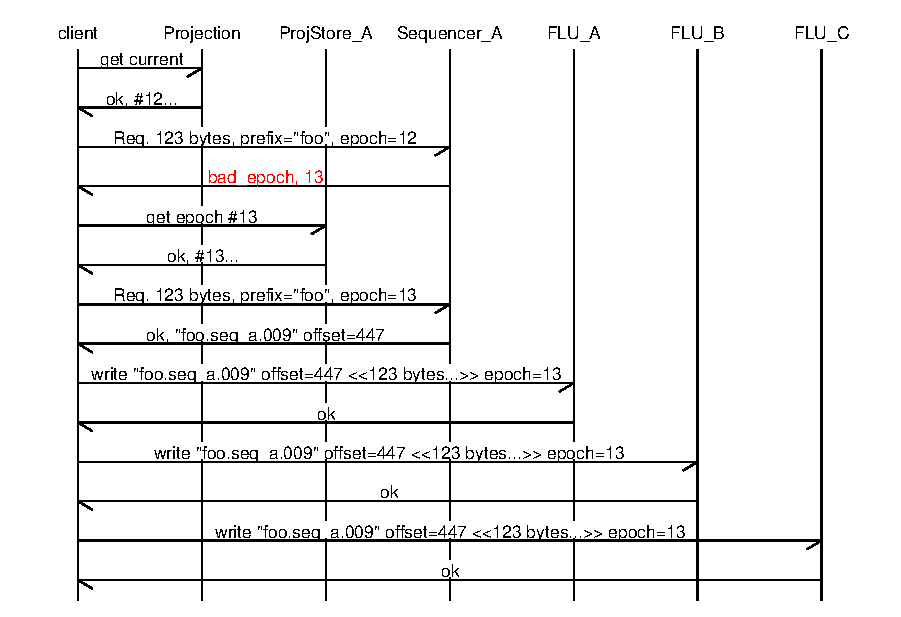
\includegraphics{append-flow}
	}
\caption{MSC diagram: append 123 bytes onto a file with prefix {\tt
    "foo"}. In error-free cases and with a correct cached projection, the
  number of network messages is $2 + 2N$ where $N$ is chain length.}
\label{fig:append-flowMSC}
\end{figure*}

\begin{figure*}[tp]
\resizebox{\textwidth}{!}{
	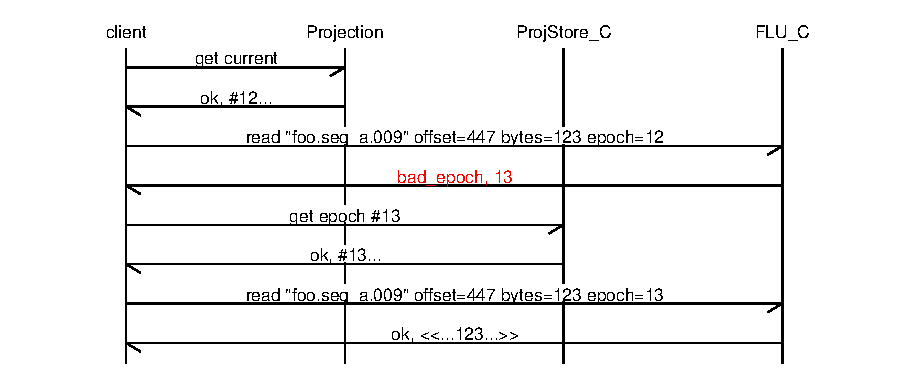
\includegraphics{read-flow}
	}
\caption{MSC diagram: read 123 bytes from a file}
\label{fig:read-flowMSC}
\end{figure*}

\begin{figure*}[tp]
\resizebox{\textwidth}{!}{
	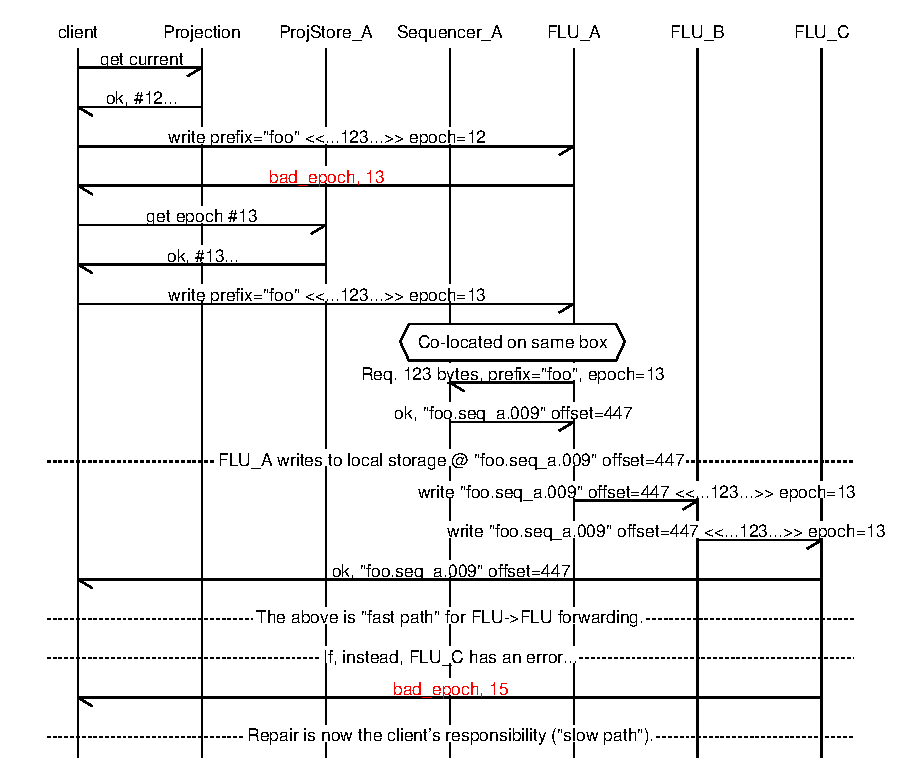
\includegraphics{append-flow2}
	}
\caption{MSC diagram: append 123 bytes onto a file with prefix {\tt
    "foo"}, using FLU$\rightarrow$FLU direct communication in original
  Chain Replication's messaging pattern.  In error-free cases and with
  a correct cached projection, the number of network messages is $N+1$
  where $N$ is chain length.}
\label{fig:append-flow2MSC}
\end{figure*}


\end{document}
